
%!TEX program = xelatex
\documentclass[letterpaper,12pt]{exam}
\usepackage{../videoNotes}
\usepackage{xcolor}
\usepackage[dvipsnames]{xcolor}
\usepackage{soul}

%\usepackage{draftwatermark}
%\SetWatermarkText{DRAFT}
%\SetWatermarkScale{1.5}
%\SetWatermarkColor{red!20}


\newcommand{\unit}{Unit 03}
\pagestyle{headandfoot}
\firstpageheader{CSC 264 \semester\ \  \unit}{}{Name: $\rule{6cm}{0.15mm}$}
\runningheader{CSC 264 \semester}{\unit}{Page \thepage\ of \numpages}
\firstpagefooter{}{}{}
\runningfooter{}{}{}

\begin{document}

%\underconstruction

\section*{\unit\_010 -- ASCII} 
\par{\fontfamily{qzc}\selectfont\textbf{Video Length 17:18 }}
\begin{questions}

\begin{samepage}
    \question What does the "A" in ASCII stand for? Why is it significant?
    \vspace{5mm}
\end{samepage}
\begin{samepage}
    \question Fill in the blanks in the following table.
\par
    \begin{tabular}
  {|c|c|c|}
  Decimal & Hex & Character \\
  \hline
  \hline
  {\Huge 0} &  &  \\
  \hline
   & {\Huge 20}  & \\
    \hline
   &  & {\Huge 0 (zero)}  \\  
  \hline
   {\Huge 64}  & &  \\
  \hline
     & {\Huge 41}  &  \\  
  \hline
   &  &  {\Huge a}  \\
  \hline
   &  & \newline {\Huge ~ (tilde)} \\
   \hline
\end{tabular}    
    \vspace{5mm}
\end{samepage}
\par
 \begin{samepage}
     \question What are the ASCII codes with values less than 32?
     \vspace{5mm}
 \end{samepage}
 \par
  \begin{samepage}
      \question If you have an uppercase letter, how can you convert it to the lower case equivalent?
      \vspace{5mm}
  \end{samepage}
  \par
   

  %%%%%%%%%%%%%%%%%%%%%%%%%%%%%%%%%%%%%%%%%%%%%%%%%%%%%
\begin{center}
    \rule{0.5\textwidth}{.4pt}
\end{center}
Do you have any questions or concerns? Please write any lingering questions you have here.
\section*{\unit\_020 -- Logic Gates }
\par{\fontfamily{qzc}\selectfont\textbf{Video Length 6:10}}
\begin{samepage}
    \question Draw the diagram for an AND gate and fill in the truth table.
    \par
    \begin{tabular}{|c|c|c|}
      |A & B & A and B \\
      \hline
      \hline
      0 & 0 &  \\
      \hline
      0 & 1 &  \\
      \hline
      1 & 0 &  \\
      \hline
      1 & 1 &  \\  
      \hline     
    \end{tabular}
    \vspace{5mm}
\end{samepage}
\begin{samepage}
    \question What is the order of the input columns on a truth table?
    \vspace{5mm}
\end{samepage}
\par
 
\begin{samepage}
    \question Draw the diagram for an OR gate and fill in the truth table.
    \par
    \begin{tabular}{|c|c|c|}
      |A & B & A or B \\
      \hline
      \hline
      0 & 0 &  \\
      \hline
      0 & 1 &  \\
      \hline
      1 & 0 &  \\
      \hline
      1 & 1 &  \\  
      \hline     
    \end{tabular}
    \vspace{5mm}
\end{samepage}
\par
\begin{samepage}
    \question Draw the diagram for an XOR gate and fill in the truth table.
    \par
    \begin{tabular}{|c|c|c|}
      |A & B & A xor B \\
      \hline
      \hline
      0 & 0 &  \\
      \hline
      0 & 1 &  \\
      \hline
      1 & 0 &  \\
      \hline
      1 & 1 &  \\  
      \hline     
    \end{tabular}
    \vspace{5mm}
\end{samepage}
\par
\begin{samepage}
    \question Draw the diagram for a NOT gate and fill in the truth table.
    \par
    \begin{tabular}{|c|c|}
      |A & not A \\
      \hline
      \hline
      0 &   \\
      \hline
      1 &   \\
      \hline    
    \end{tabular}
    \vspace{5mm}
\end{samepage}
\begin{samepage}
    \question Draw the diagram for an NAND gate and fill in the truth table.
    \par
    \begin{tabular}{|c|c|c|}
      |A & B & A nand B \\
      \hline
      \hline
      0 & 0 &  \\
      \hline
      0 & 1 &  \\
      \hline
      1 & 0 &  \\
      \hline
      1 & 1 &  \\  
      \hline     
    \end{tabular}
    \vspace{5mm}
\end{samepage}
\begin{samepage}
    \question Draw the diagram for an NOR gate and fill in the truth table.
    \par
    \begin{tabular}{|c|c|c|}
      |A & B & A nor B \\
      \hline
      \hline
      0 & 0 &  \\
      \hline
      0 & 1 &  \\
      \hline
      1 & 0 &  \\
      \hline
      1 & 1 &  \\  
      \hline     
    \end{tabular}
    \vspace{5mm}
\end{samepage}
\begin{samepage}
    \question Explain the difference between a NOR gate and an XOR gate
    \vspace{5mm}
\end{samepage}
\par
 
\par
\rule{0.5\textwidth}{.4pt} %End of section
\section*{\unit\_030 -- Adders}
\par{\fontfamily{qzc}\selectfont\textbf{Video Length 15:00}}
\begin{samepage}
    \question Add the binary numbers 0b00101011 + 0b00111101.  Check your answer by converting the numbers to decimal.
    \vspace{5mm}
\end{samepage}
\par
\begin{samepage}
    \question What is the difference between a half adder and a full adder?
    \vspace{5mm}
\end{samepage}
\par
\begin{samepage}
    \question Fill in the truth table for a full adder.
    \par 

    \begin{tabular}{|c|c|c|c|c|}
      \hline
      A & B & $C{in}$ & Sum & $C{out}$ \\
      \hline
      \hline
       &  &  &  &  \\
      \hline
       &  &  &  &  \\
      \hline
      0 & 1 & 0 &  &  \\
      \hline
       &  &  &  &  \\
      \hline
       &  &  &  &  \\
      \hline
      1 & 0 & 1 &  &  \\
      \hline
       &  &  &  &  \\
      \hline
       &  &  &  &  \\  
      \hline
      
    \end{tabular}

    \vspace{5mm}
\end{samepage}
\par
  
\rule{0.5\textwidth}{.4pt} %End of section
%----------------------------------
\section*{\unit\_040 -- Suffixes }
\par{\fontfamily{qzc}\selectfont\textbf{Video Length 20:00 }}
\begin{samepage}
    \question What is the suffix for an instruction that works on 64 bit registers?  What is an example of a 64 bit register?

    \vspace{5mm}
\end{samepage}
\par
\begin{samepage}
    \question What is the suffix for an instruction that works on 32 bit registers?  What is an example of a 32 bit register?     
    \vspace{5mm}
\end{samepage}
\par
\begin{samepage}
    \question What is the suffix for an instruction that works on 16 bit registers?  What is an example of a 16 bit register?     
    \vspace{5mm}
\end{samepage}
\par
\begin{samepage}
    \question What is the suffix for an instruction that works on an 8 bit registers?  What is an example of an 8 bit register?
    \vspace{5mm}
\end{samepage}
\par
\begin{samepage}
    \question What would the content of the RAX register be after executing the following code?
    \begin{verbatim}
         movq $0x7fffffffffffffff, %rax
         movw $0, %ax      
    \end{verbatim}
    \vspace{5mm}
\end{samepage}
\par
 \par
\begin{samepage}
    \question What would the content of the RAX register be after executing the following code?
    \begin{verbatim}
         movq $0x7fffffffffffffff, %rax
         movl $0, %eax      
    \end{verbatim}
    \vspace{5mm}
\end{samepage}
\rule{0.5\textwidth}{.4pt} %End of section
%----------------------------------
\section*{\unit\_050 -- XOR}
\par{\fontfamily{qzc}\selectfont\textbf{Video Length 20:00 }}
\begin{samepage}
    \question Write the code needed to clear the RAX register using XOR.
    \vspace{5mm}
\end{samepage}
\par
\begin{samepage}
    \question Why is using XOR to clear a register better than using MOV?
    \vspace{5mm}
\end{samepage}
\par
\section*{\unit\_060 -- Add}
\par{\fontfamily{qzc}\selectfont\textbf{Video Length 3:45}}
\begin{samepage}
    \question  Cross out the instructions that are invalid.  Put a check mark next to the ones that are valid.  (You may assume that the data fields are valid)
\begin{verbatim}
      addq %rax, %rbx

      addq %rax, %r9
      
      addq num1, %rdi 
      
      addq num1, num2
      
      addq $17, %rcx
      
      addq $17, num1
      
      addq $rcx, num1 
\end{verbatim}
    \vspace{5mm}
\end{samepage}
\par
\rule{0.5\textwidth}{.4pt} %End of section
%---------------------------------- 
\rule{0.5\textwidth}{.4pt} %End of section
%----------------------------------
\section*{\unit\_070, Part 1 -- Complements}
\par{\fontfamily{qzc}\selectfont\textbf{Video Length 7:20}}
\begin{samepage}
    \question What arithmetic operation is complement arithmetic used for?
    \vspace{5mm}
\end{samepage}
\par
\begin{samepage}
    \question What is the ten's complement of 7?
    \vspace{5mm}
\end{samepage}
\par
\rule{0.5\textwidth}{.4pt} %End of section
%----------------------------------
\section*{\unit\_070 Part 2 -- Complements}
\par{\fontfamily{qzc}\selectfont\textbf{Video Length 9:25}}
\begin{samepage}
    \question What is the rule for converting a binary number into its two's complement?
    \vspace{5mm}
\end{samepage}
\par
    \question What is the two's complement of the binary number 0b00001101?
    \vspace{5mm}
    \question How can you tell if a binary number is negative?
    \vspace{5mm}
     \question What is the rule for converting a two's complement number back to a positive value?
     \vspace{5mm}
     \question What is the range of possible values for a signed byte?
     \vspace{5mm}
 \section*{\unit\_070 Part 3 -- Complements }
 \par{\fontfamily{qzc}\selectfont\textbf{Video Length 9:25}}
 \begin{samepage}
     \question Do the subtraction problem 0b00101100 - 0b00010111 using two's complement arithmetic.  Show all your work.
     \vspace{40mm}
 \end{samepage}
 \par
 \rule{0.5\textwidth}{.4pt} %End of section
 %----------------------------------  

 \section*{\unit\_070 Part 3 -- Complements }
 \par{\fontfamily{qzc}\selectfont\textbf{Video Length 4:40}}
 \begin{samepage}
     \question Why do computers use two's complement arithmetic instead of one's complement arithmetic?
     \vspace{15mm}
 \end{samepage}
 \par

\begin{samepage}
    \question Assume you have 'num1', 'num2', and 'difference' defined with quad values.  Write the code needed to subtract num2 from num 1 and store the result in difference.
    \vspace{5mm}
\end{samepage}
\par
 

%----------------------------------
\end{questions} 
%footer
\vfill
\begin{center}
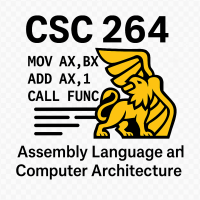
\includegraphics{../csc264Logo}
\end{center}
\end{document} 